
%%%%%%%%%%%%%%%%%%%%%%%%%%%%%%%%%%%%%%%%%%%%%%%%%%%%%%%%
\documentclass[12pt,a4paper]{article}% 文档格式
\usepackage{ctex,hyperref}% 输出汉字
\usepackage{times}% 英文使用Times New Roman
%%%%%%%%%%%%%%%%%%%%%%%%%%%%%%%%%%%%%%%%%%%%%%%%%%%%%%%%
\title{\fontsize{18pt}{27pt}\selectfont% 小四字号,1.5倍行距
	{\heiti% 黑体 
		Physics Homework}}% 题目
%%%%%%%%%%%%%%%%%%%%%%%%%%%%%%%%%%%%%%%%%%%%%%%%%%%%%%%%
\author{\fontsize{12pt}{18pt}\selectfont% 小四字号,1.5倍行距
	{\fangsong% 仿宋
		Haixuan Lin}\\% 标题栏脚注
	\fontsize{10.5pt}{15.75pt}\selectfont% 五号字号,1.5倍行距
	{\fangsong% 仿宋
		(Fudan University department of physics
		)}}% 作者单位,“~”表示空格
%%%%%%%%%%%%%%%%%%%%%%%%%%%%%%%%%%%%%%%%%%%%%%%%%%%%%%%%
\date{}% 日期(这里避免生成日期)
%%%%%%%%%%%%%%%%%%%%%%%%%%%%%%%%%%%%%%%%%%%%%%%%%%%%%%%%
\usepackage{amsmath,amsfonts,amssymb}% 为公式输入创造条件的宏包
%%%%%%%%%%%%%%%%%%%%%%%%%%%%%%%%%%%%%%%%%%%%%%%%%%%%%%%%
\usepackage{graphicx}% 图片插入宏包
\usepackage{subfigure}% 并排子图
\usepackage{float}% 浮动环境,用于调整图片位置
\usepackage[export]{adjustbox}% 防止过宽的图片
\usepackage{pdfpages}
%%%%%%%%%%%%%%%%%%%%%%%%%%%%%%%%%%%%%%%%%%%%%%%%%%%%%%%%
\usepackage{bibentry}
\usepackage{natbib}% 以上2个为参考文献宏包
%%%%%%%%%%%%%%%%%%%%%%%%%%%%%%%%%%%%%%%%%%%%%%%%%%%%%%%%
\usepackage{abstract}% 两栏文档,一栏摘要及关键字宏包
\renewcommand{\abstracttextfont}{\fangsong}% 摘要内容字体为仿宋
\renewcommand{\abstractname}{\textbf{摘\quad 要}}% 更改摘要二字的样式
%%%%%%%%%%%%%%%%%%%%%%%%%%%%%%%%%%%%%%%%%%%%%%%%%%%%%%%%
\usepackage{xcolor}% 字体颜色宏包
\newcommand{\red}[1]{\textcolor[rgb]{1.00,0.00,0.00}{#1}}
\newcommand{\blue}[1]{\textcolor[rgb]{0.00,0.00,1.00}{#1}}
\newcommand{\green}[1]{\textcolor[rgb]{0.00,1.00,0.00}{#1}}
\newcommand{\darkblue}[1]
{\textcolor[rgb]{0.00,0.00,0.50}{#1}}
\newcommand{\darkgreen}[1]
{\textcolor[rgb]{0.00,0.37,0.00}{#1}}
\newcommand{\darkred}[1]{\textcolor[rgb]{0.60,0.00,0.00}{#1}}
\newcommand{\brown}[1]{\textcolor[rgb]{0.50,0.30,0.00}{#1}}
\newcommand{\purple}[1]{\textcolor[rgb]{0.50,0.00,0.50}{#1}}% 为使用方便而编辑的新指令
\renewcommand{\d}{\mathrm{d}}
%%%%%%%%%%%%%%%%%%%%%%%%%%%%%%%%%%%%%%%%%%%%%%%%%%%%%%%%
\usepackage{url}% 超链接
\usepackage{bm}% 加粗部分公式
\usepackage{multirow}
\usepackage{booktabs}
\usepackage{epstopdf}
\usepackage{epsfig}
\usepackage{longtable}% 长表格
\usepackage{supertabular}% 跨页表格
\usepackage{algorithm}
\usepackage{algorithmic}
\usepackage{changepage}% 换页
%%%%%%%%%%%%%%%%%%%%%%%%%%%%%%%%%%%%%%%%%%%%%%%%%%%%%%%%
\usepackage{enumerate}% 短编号
\usepackage{caption}% 设置标题
\captionsetup[figure]{name=\fontsize{10pt}{15pt}\selectfont Figure}% 设置图片编号头
\captionsetup[table]{name=\fontsize{10pt}{15pt}\selectfont Table}% 设置表格编号头
%%%%%%%%%%%%%%%%%%%%%%%%%%%%%%%%%%%%%%%%%%%%%%%%%%%%%%%%
%\usepackage{indentfirst}% 中文首行缩进
\usepackage[left=2.50cm,right=2.50cm,top=2.80cm,bottom=2.50cm]{geometry}% 页边距设置
\renewcommand{\baselinestretch}{1.5}% 定义行间距(1.5)
%%%%%%%%%%%%%%%%%%%%%%%%%%%%%%%%%%%%%%%%%%%%%%%%%%%%%%%%
\usepackage{fancyhdr} %设置全文页眉、页脚的格式
\pagestyle{fancy}
\hypersetup{colorlinks=true,linkcolor=black}% 去除引用红框,改变颜色
%%%%%%%%%%%%%%%%%%%%%%%%%%%%%%%%%%%%%%%%%%%%%%%%%%%%%%%%
\usepackage{caption}%标题取消自动figure
\usepackage{multicol}
\usepackage{cuted}
%%%%%%%%%%%%%%%%%%%%%%%%%%%%%%%%%%%%%%%%%%%%%%%%%%%%%%%%
\newcommand{\nonumbersection}[1]{
	\section*{#1}
	\addcontentsline{toc}{section}{#1}
}
\newcommand{\nonumbersubsection}[1]{
	\subsection*{#1}
	\addcontentsline{toc}{subsection}{#1}
}
%%%%%%%%%%%%%%%%%%%%%%%%%%%%%%%%%%%%%%%%%%%%%%%%%%%%%%%%
\begin{document}% 以下为正文内容
	\maketitle% 产生标题,没有它无法显示标题
	%%%%%%%%%%%%%%%%%%%%%%%%%%%%%%%%%%%%%%%%%%%%%%%%%%%%%%%%
	\lhead{}% 页眉左边设为空
	\chead{}% 页眉中间设为空
	\rhead{}% 页眉右边设为空
	\lfoot{}% 页脚左边设为空
	\cfoot{\thepage}% 页脚中间显示页码
	\rfoot{}% 页脚右边设为空
	%%%%%%%%%%%%%%%%%%%%%%%%%%%%%%%%%%%%%%%%%%%%%%%%%%%%%%%%
	
	
	\begin{center}% 居中处理
		{\textbf{Abstract}}% 英文摘要
	\end{center}
	\begin{adjustwidth}{1.06cm}{1.06cm}% 英文摘要内容
		\hspace{1.5em}In order to improve my computer and English skills, please allow me to complete this physics homework in English context with \LaTeX, so as to improve my professional level. Sorry for the inconvenience!
	\end{adjustwidth}
	
	\newpage% 从新的一页继续
	
	\renewcommand{\contentsname}{Contents}
	\tableofcontents
	\newpage

\nonumbersection{Question 10-3}
\noindent Calculate time in the Earth reference frame.
\begin{equation}
	t=\frac{S}{v}
\end{equation}
According to the clock slowing effect, the time in the spacecraft's reference frame is.
\begin{equation}
	t'=\frac{S}{v}\sqrt{1-\dfrac{v^2}{c^2}}
\end{equation}
So.
\begin{equation}
	\Delta t =t-t'
\end{equation}
The solution is.
\begin{equation}
	v=\dfrac{\dfrac{2\Delta t}{S}}{\dfrac{\Delta t^2}{S^2}+\dfrac{1}{c^2}}\approx0.198c\approx5.932\times10^7\ \mathrm{m/s}
\end{equation}
Note that here we consider $c=299792458\ \mathrm{m/s}$.
\nonumbersection{Question 10-7}
\nonumbersubsection{(1)}
\noindent As far as the people in the carriage are concerned, the length of the car is constant.
$$
\Delta t_1'=\frac{L}{c}
$$
$$
\Delta t'=\frac{2L}{c}
$$
\nonumbersubsection{(2)}
\noindent According to the scaling effect, the observer in the ground will measure the car's length as below.
\begin{equation}
	L'=L\sqrt{1-\dfrac{v^2}{c^2}}
\end{equation}
The photon is chasing the right end of the car.
 \begin{equation}
 	L'+v\Delta t_1=c\Delta t_1
 \end{equation}
 The solution is.
 $$
 \Delta t_1=\frac{L}{c}\sqrt{\dfrac{c+v}{c-v}}
 $$
 According to the clock slowing effect.
 $$
 \Delta t=\dfrac{\Delta t'}{\sqrt{1-\dfrac{v^2}{c^2}}}=\frac{2L}{c}\dfrac{1}{\sqrt{1-\dfrac{v^2}{c^2}}}
 $$
 \nonumbersection{Question 10-9}
 \nonumbersubsection{(1)}
 \noindent According to symmetry analysis, the two observers would have the opposite situation. B 棒上的观察者会看到两棒右端先重合,再左端重合.
 \nonumbersubsection{(2)}
 \noindent According to the scaling effect.
 \begin{equation}
 	l'=l_0\sqrt{1-\dfrac{v^2}{c^2}}
 \end{equation}
 A simple kinematic formula is obtained.
 \begin{equation}
 	l_0-l'=v\Delta t
 \end{equation}
 We solve that.
 $$
 v=\dfrac{\dfrac{2\Delta t}{l_0}}{\dfrac{\Delta t^2}{l_0^2}+\dfrac{1}{c^2}}
 $$
 \nonumbersection{(3)}
 \noindent According to symmetry analysis, the two observers would have the opposite situation. 两个端点同时重合.
 \nonumbersection{Question 10-12}
 \noindent According to the clock slowing effect.
 \begin{equation}
 	v=\dfrac{1}{\sqrt{\dfrac{t_0^2}{S^2}+\dfrac{1}{c^2}}}\approx0.998c\approx2.997\times10^8\ \mathrm{m/s}
 \end{equation}
 \nonumbersection{Question 10-17}
 \nonumbersubsection{(1)}
 \noindent The length of the projection of the rod in the y direction is constant, define it as $H$. According to the Lorentz transformation.
 \begin{equation}
 	v_{S'}^{\left( O \right)}=\dfrac{v_{S'}^{(S)}-v_{S'}^{(S)}}{1-\dfrac{v_{S'}^{(S)}v_{S'}^{(S)}}{c^2}}=\dfrac{0.6c-v}{1-\dfrac{0.6v}{c}} 	
 \end{equation}
 Based on simple geometry and scaling effect.
 \begin{equation}
 	L_{x}^{(S)}=H\cot \theta ^{(S)}=H\cot 45^{\circ}=L_{x}^{(O)}\sqrt{1-\left[ \frac{v_{S}^{(O)}}{c} \right] ^2}
 \end{equation}
 \begin{equation}
 	L_{x}^{(S')}=H\cot \theta ^{(S')}=H\cot 35^{\circ}=L_{x}^{(O)}\sqrt{1-\left[ \frac{v_{S'}^{(O)}}{c} \right] ^2}
 \end{equation}
 And we know $v_{S'}^{(O)}=v$, so we get.
 \begin{equation}
 	\left( \dfrac{\cot 45^{\circ}}{\cot 35^{\circ}} \right) ^2=\dfrac{1-\left( \dfrac{v}{c} \right) ^2}{1-\left( \dfrac{0.6-\dfrac{v}{c}}{1-\dfrac{0.6v}{c}} \right) ^2}
 \end{equation}
 This is a quartic equation with one variable, the analytical solution is very complex, but the numerical solution can be calculated.
 $$
 v_O^{(S)}=v\approx0.73c
 $$
 
 
 \nonumbersubsection{(2)}
 \noindent Solve the euqations above we can get.
 $$
 v_{O}^{(S')}\approx0.24c
 $$
 \nonumbersubsection{(3)}
 \noindent Do a tansformation of equation above.
 \begin{equation}
 	L_{x}^{(S)}=H\cos \theta ^{(S)}=L_{x}^{(O)}\sqrt{1-\dfrac{v^2}{c^2}}=H\cos \theta ^{(O)}\sqrt{1-\dfrac{v^2}{c^2}}
 \end{equation}
 As a result.
 $$
 \theta^{(O)}=\arctan\left( \tan\theta^{(O)}\sqrt{1-\dfrac{v^2}{c^2}}\right) \approx34.2^\circ
 $$
 \nonumbersection{Question 10-18}
 \nonumbersubsection{(1)}
 \noindent By symmetry analysis.
 $$
 v_B^{(A)}=v_A^{(B)}=0.7c
 $$
 It is easily obtained by the Lorentz transformation.
 $$
 v_C^{(A)}=\dfrac{v_C^{(B)}-v_A^{(B)}}{1-\dfrac{v_C^{(B)}v_A^{(B)}}{c^2}}=\frac{140}{149}c\approx0.94c
 $$
 
 \nonumbersubsection{(2)}
 \noindent It is easily obtained by the Lorentz transformation.
$$
v_{A}^{(O)}=\dfrac{v_{A}^{(B)}+v_{B}^{(O)}}{1+\dfrac{v_{A}^{(B)}v_{B}^{(O)}}{c^2}}=\dfrac{20}{37}c\approx0.54c
$$
 $$
 v_{C}^{(O)}=\dfrac{v_{C}^{(B)}+v_{B}^{(O)}}{1+\dfrac{v_{C}^{(B)}v_{B}^{(O)}}{c^2}}=\dfrac{160}{163}c\approx 0.98c
 $$
 \nonumbersection{Question 10-27}
 \noindent According to the mass-energy equation.
 \begin{equation}
 	E_{\mathrm{k}}=mc^2-m_0c^2=m_0c^2\left( \frac{1}{\sqrt{1-\dfrac{v^2}{c^2}}}-1 \right) =\dfrac{1}{2}m_0c^2
 \end{equation}
 So.
 $$
 v=\frac{\sqrt{5}}{3}c\approx2.2\times10^8\ \mathrm{m/s}
 $$
 \nonumbersection{Question 10-30}
 \noindent According to the law of conservation of momentum and conservation of energy.
 \begin{equation}
 	p_0=Mv_M
 \end{equation}
 \begin{equation}
 	m_0c^2+4m_0c^2=Mv_M^2
 \end{equation}
 And we know that.
 \begin{equation}
 	4m_0c^2=\dfrac{m_0c^2}{\sqrt{1-\dfrac{v_m^2}{c^2}}}
 \end{equation}
 \begin{equation}
 	p_0=mv_m=\dfrac{m_0v}{\sqrt{1-\dfrac{v_m^2}{c^2}}}
 \end{equation}
 According to quality and efficiency.
 \begin{equation}
 	M=\dfrac{M_0}{\sqrt{1-\dfrac{v_M^2}{c^2}}}
 \end{equation}
 The solution is.
 $$
 M_0=\sqrt{10}m_0\approx3.16m_0
 $$
 \nonumbersection{Question 10-31}
 \nonumbersubsection{(1)}
 \begin{figure}[h]
 	\centering
 	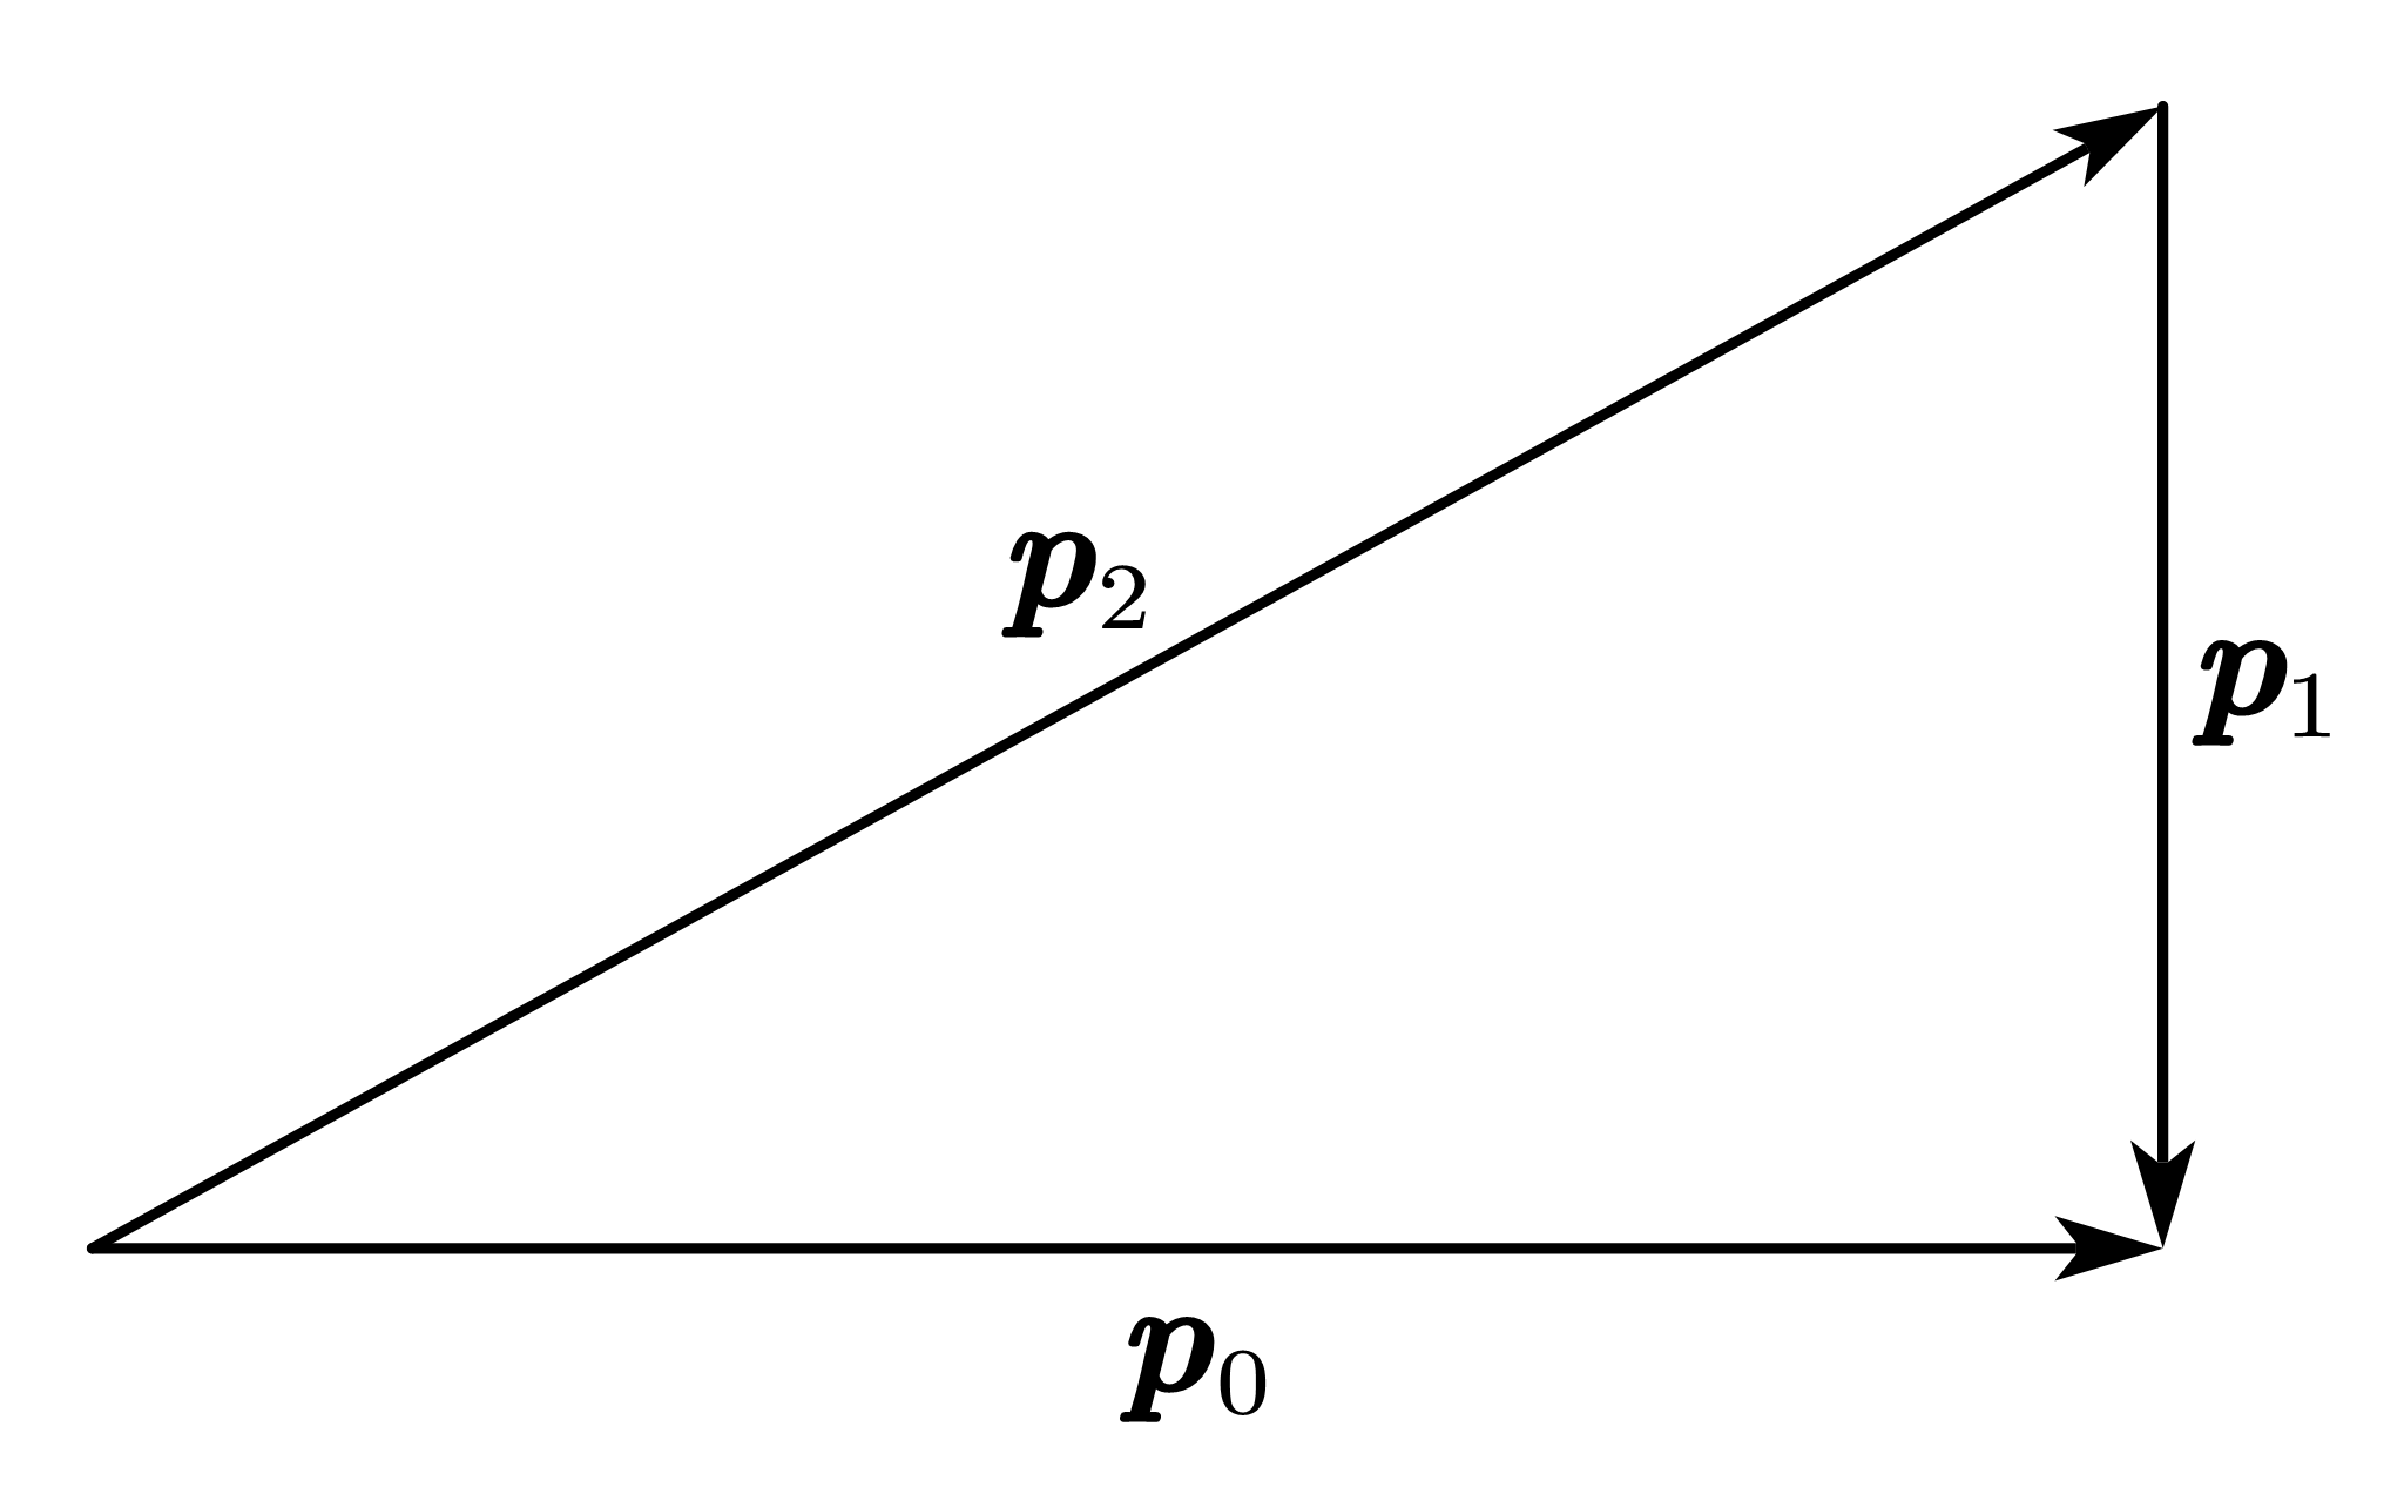
\includegraphics[width=0.7\linewidth]{10-31}
 	\caption*{}
 	\label{fig:10-31}
 \end{figure}
 
 \noindent According to the Lorentz transformation.
 \begin{equation}
 	p_0=m'v'=\dfrac{m_0'}{\sqrt{1-\dfrac{0.8^2c^2}{c^2}}}0.8c=\dfrac{4}{3}m_0'c
 \end{equation}
 \begin{equation}
 	p_1=m_1v_1=\dfrac{m_0}{\sqrt{1-\dfrac{0.6^2c^2}{c^2}}}0.6c=\dfrac{3}{4}m_0c 
 \end{equation}
 \begin{equation}
 	p_2=m_2v_2=\dfrac{m_0}{\sqrt{1-\dfrac{v^2}{c^2}}}v
 \end{equation}
 According to the Pythagorean theorem.
 \begin{equation}
 	p_2^2=p_0^2+p_1^2
 \end{equation}
 At the same time, the energy is also conservative.
 \begin{equation}
 	E_0=E_1+E_2
 \end{equation}
 The Lorentz transformation tells us.
 \begin{equation}
 	E_0=\dfrac{m_0'c^2}{\sqrt{1-\dfrac{0.8^2c^2}{c^2}}}=\dfrac{5}{3}m_0'c^2
 \end{equation}
 \begin{equation}
 	E_1=\dfrac{m_0c^2}{\sqrt{1-\dfrac{0.6^2c^2}{c^2}}}=\dfrac{5}{4}m_0c^2
 \end{equation}
 \begin{equation}
 	E_2=\sqrt{m_0^2c^4+p_2^2c^2}
 \end{equation}
 We solve this.
 $$
 v=\sqrt{\dfrac{40729}{42025}}c\approx0.984c
 $$
 $$
 \theta =\arctan\dfrac{p_1}{p_0}=\arctan\dfrac{27}{200}=\arctan0.135
 $$
 \nonumbersubsection{(2)}
 We solve it above.
 $$
 \dfrac{m_0}{m_0'}=\dfrac{6}{25}\approx0.24
 $$
 \nonumbersection{Question 10-32}
 \noindent The moment is conservative.
 \begin{equation}
 	p_\gamma=p_{\mathrm{ship}}=\dfrac{m_0'}{\sqrt{1-\dfrac{0.6^2c^2}{c^2}}}0.6c
 \end{equation}
 The energy of photon is.
 \begin{equation}
 	E_\gamma = p_\gamma c
 \end{equation}
 The energy of moving ship is.
 \begin{equation}
 	E_{\mathrm{ship}}=\dfrac{m_0'}{\sqrt{1-\dfrac{0.6^2c^2}{c^2}}}c^2
 \end{equation}
 The energy is conservative.
 \begin{equation}
 	E_\gamma + E_{\mathrm{ship}} = m_0c^2
 \end{equation}
 As a result.
 $$
 \dfrac{m_0'}{m_0}=\frac{1}{2}
 $$
\end{document}